\section{Conclusion}
The Standard Model of particle physics is the best theoretical framework so far to describe the nature around us. Although severely experimentally tested, this theory has its shortcomings and can not explain phenomena such as neutrino masses, dark matter, or dark energy. The heaviest particles in the Standard Model is the top quark , leading to the believe that it has an enhanced sensitivity to various new particles and interactions suggested by beyond the Standard Model theories. The top quark decays almost exclusively to a \PW\ boson and a bottom quark with a very short lifetime, making it escape from any bound states. This makes it possible to directly study the top quark properties by analysing its decay products, making the top quark a preferred candidate to study new physics phenomena. The Large Hadron Collider is a proton collider, producing a large number of events containing top quarks. At the proton collision points, experiments are placed to study the collisions. The search presented in this thesis is performed on data collected by the Compact Muon Solenoid experiment at a centre-of-mass energy of 13~\TeV, resulting in 35.9~\fbinv\ of integrated luminosity. 


Flavour changing neutral currents are forbidden at tree level and  highly suppressed at higher order in the Standard Model. Nonetheless, many beyond the Standard Model theories enhance their probability. In this thesis, a search in three lepton final states is performed for the production of single top quarks via the \tZq\ vertex, with $\Pquark=\Pcharm, \Pup$, or in the top quark pair processes where one of the top quarks decays through this vertex.  No significant deviation with respect to the predicted background is observed and upper limits at 95\% confidence level are placed. The observed (expected) upper limits at 95$\%$ confidence level  on the branching fractions of top quark decays are: $\BR(\Ptop \rightarrow \Pup\PZ) < 2.4\times 10^{-4}$ ($1.5\times 10^{-4}$) and $\BR(\Ptop \rightarrow \Pcharm\PZ) < 4.5\times 10^{-4}$ (3.7$\times 10^{-4}$), assuming one non-vanishing coupling at a time. A summary of the observed (expected) limits on the FCNC \tZq\ vertex is shown in \fig{fig:zoom}. 
\begin{figure}[htbp]
	\centering
	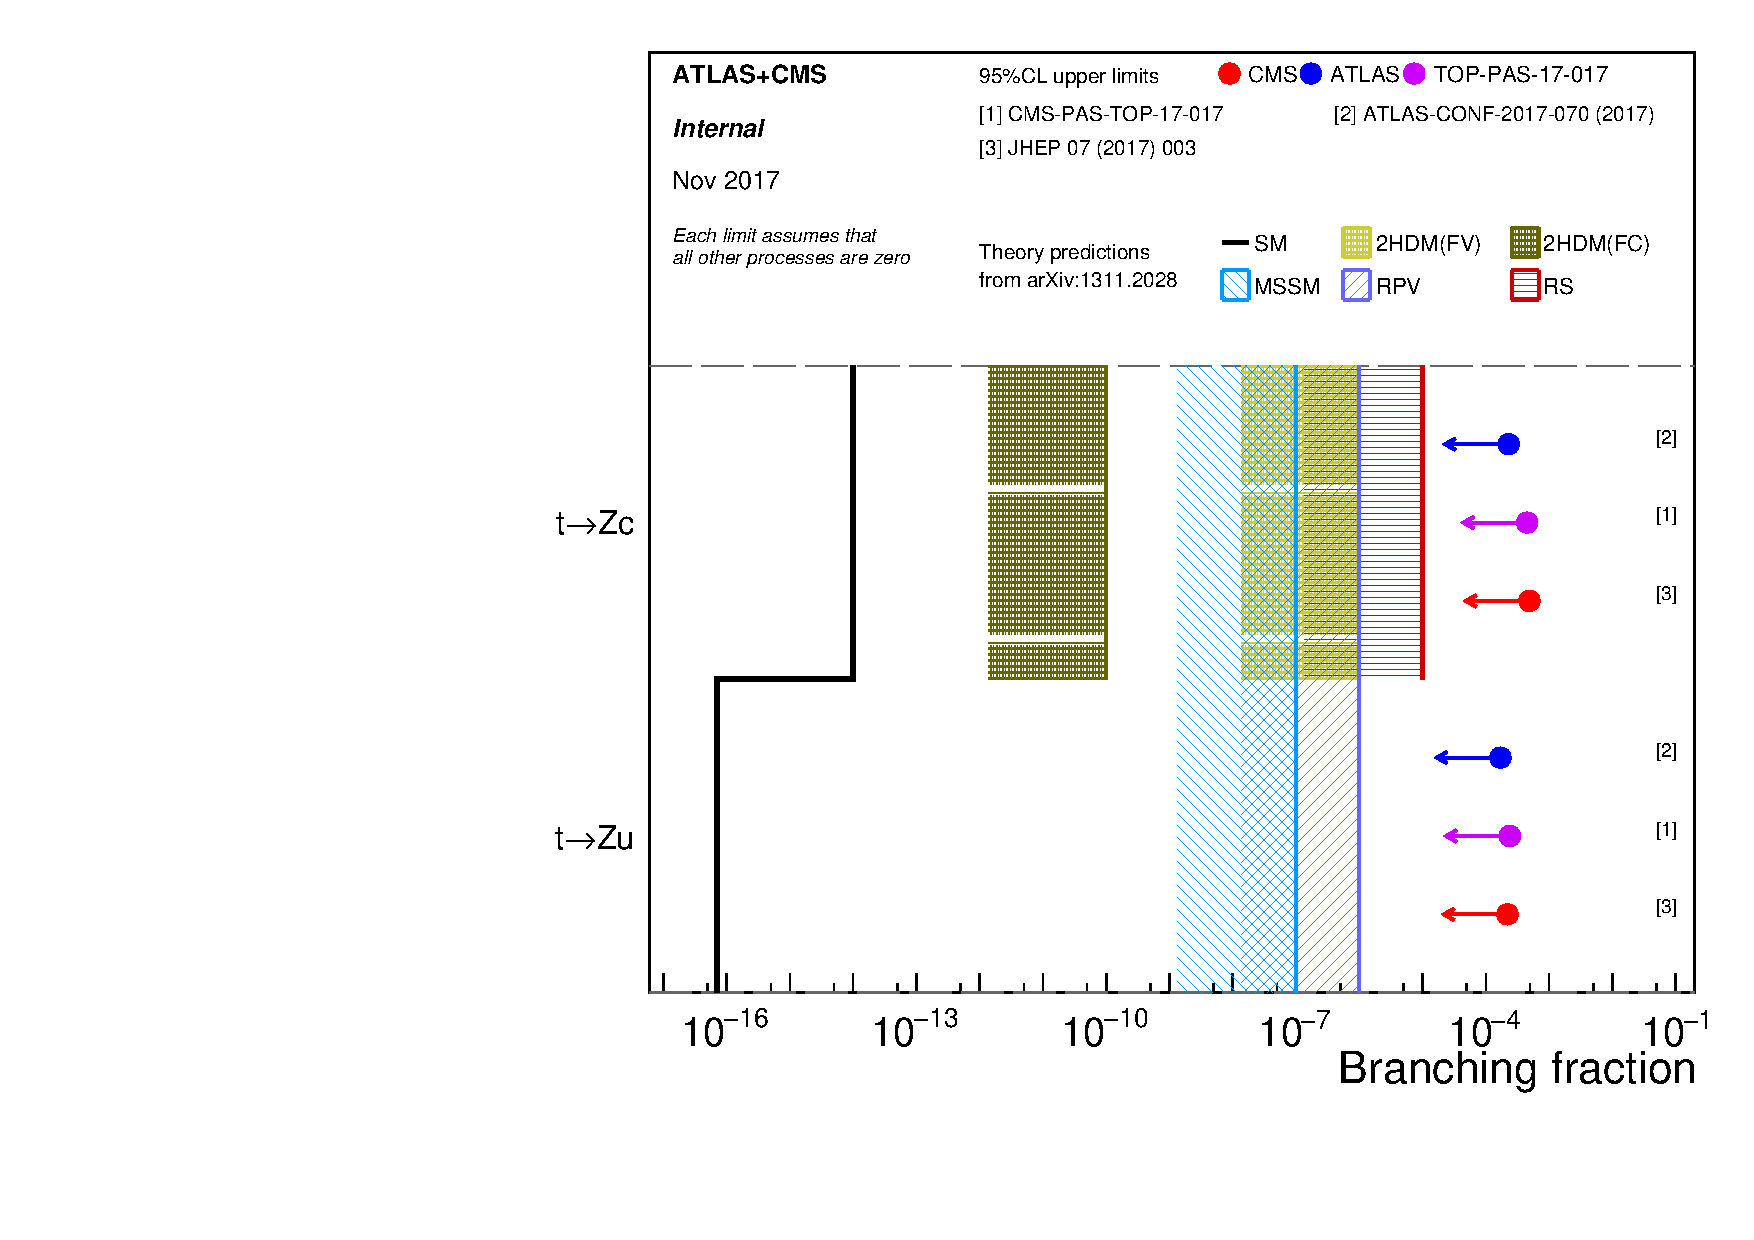
\includegraphics[width=0.49\linewidth]{7_Conclusion/Figures/fcnc_upperlimitszoom.pdf}
	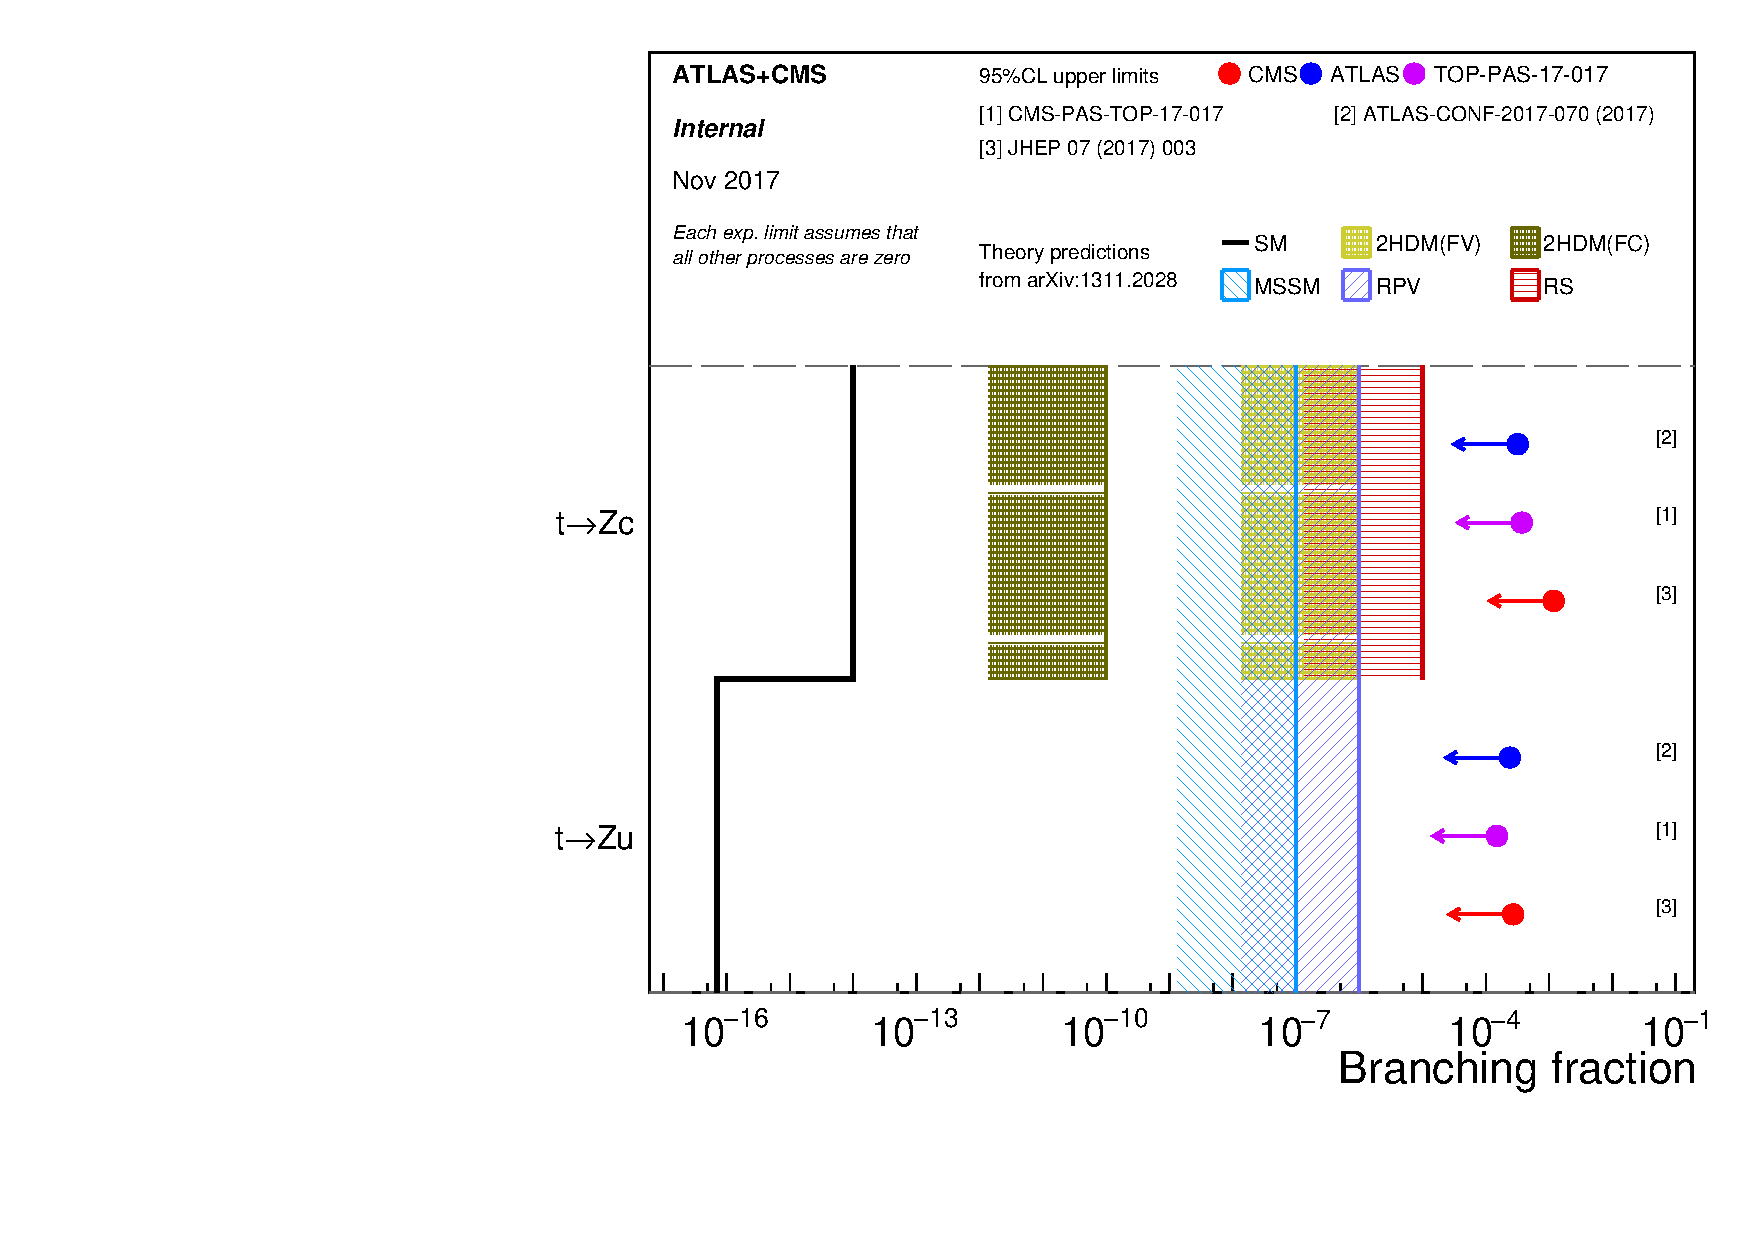
\includegraphics[width=0.49\linewidth]{7_Conclusion/Figures/fcnc_upperlimitszoomexp.pdf}
	\caption{Summary of the most stringent observed (left) and expected (right) upper limits on FCNC \tZq\ at 95\% CL upper limits from CMS (red) and ATLAS (blue) at a centre-of-mass of 8 and 13 \TeV. The results from this thesis are shown in purple. A comparison between theory predictions and experimental limits is shown. Figure adapted from \cite{summarywiki}.}
	\label{fig:zoom}
\end{figure}

Significant improvements are developed with respect to previous searches, namely by using other kinematic variables as input into the BDT as well as a better handle on the \NPL\ background.  The expected limit for the FCNC \Zut\ interaction is more stringent than the expected limit of 2.4$\times 10^{-4}$ for the current  most stringent observedlimit of 1.7$\times 10^{-4}$, set at a centre-of-mass energy of 13~\TeV\ by the ATLAS collaboration~\cite{ATLAS-CONF-2017-070}.  The  observed (expected) limit on the \Zct\ interaction set by ATLAS is 2.3$\times 10^{-4}$ (3.2$\times 10^{-4}$) and its expected limit is comparable with the expected limit presented  in this search.  For the FCNC interactions with a \tZq\ vertex, the branching fractions predicted within the Standard Model or beyond the Standard Model theories are still out of reach. 
%\begin{figure}[htbp]
%	\centering
%	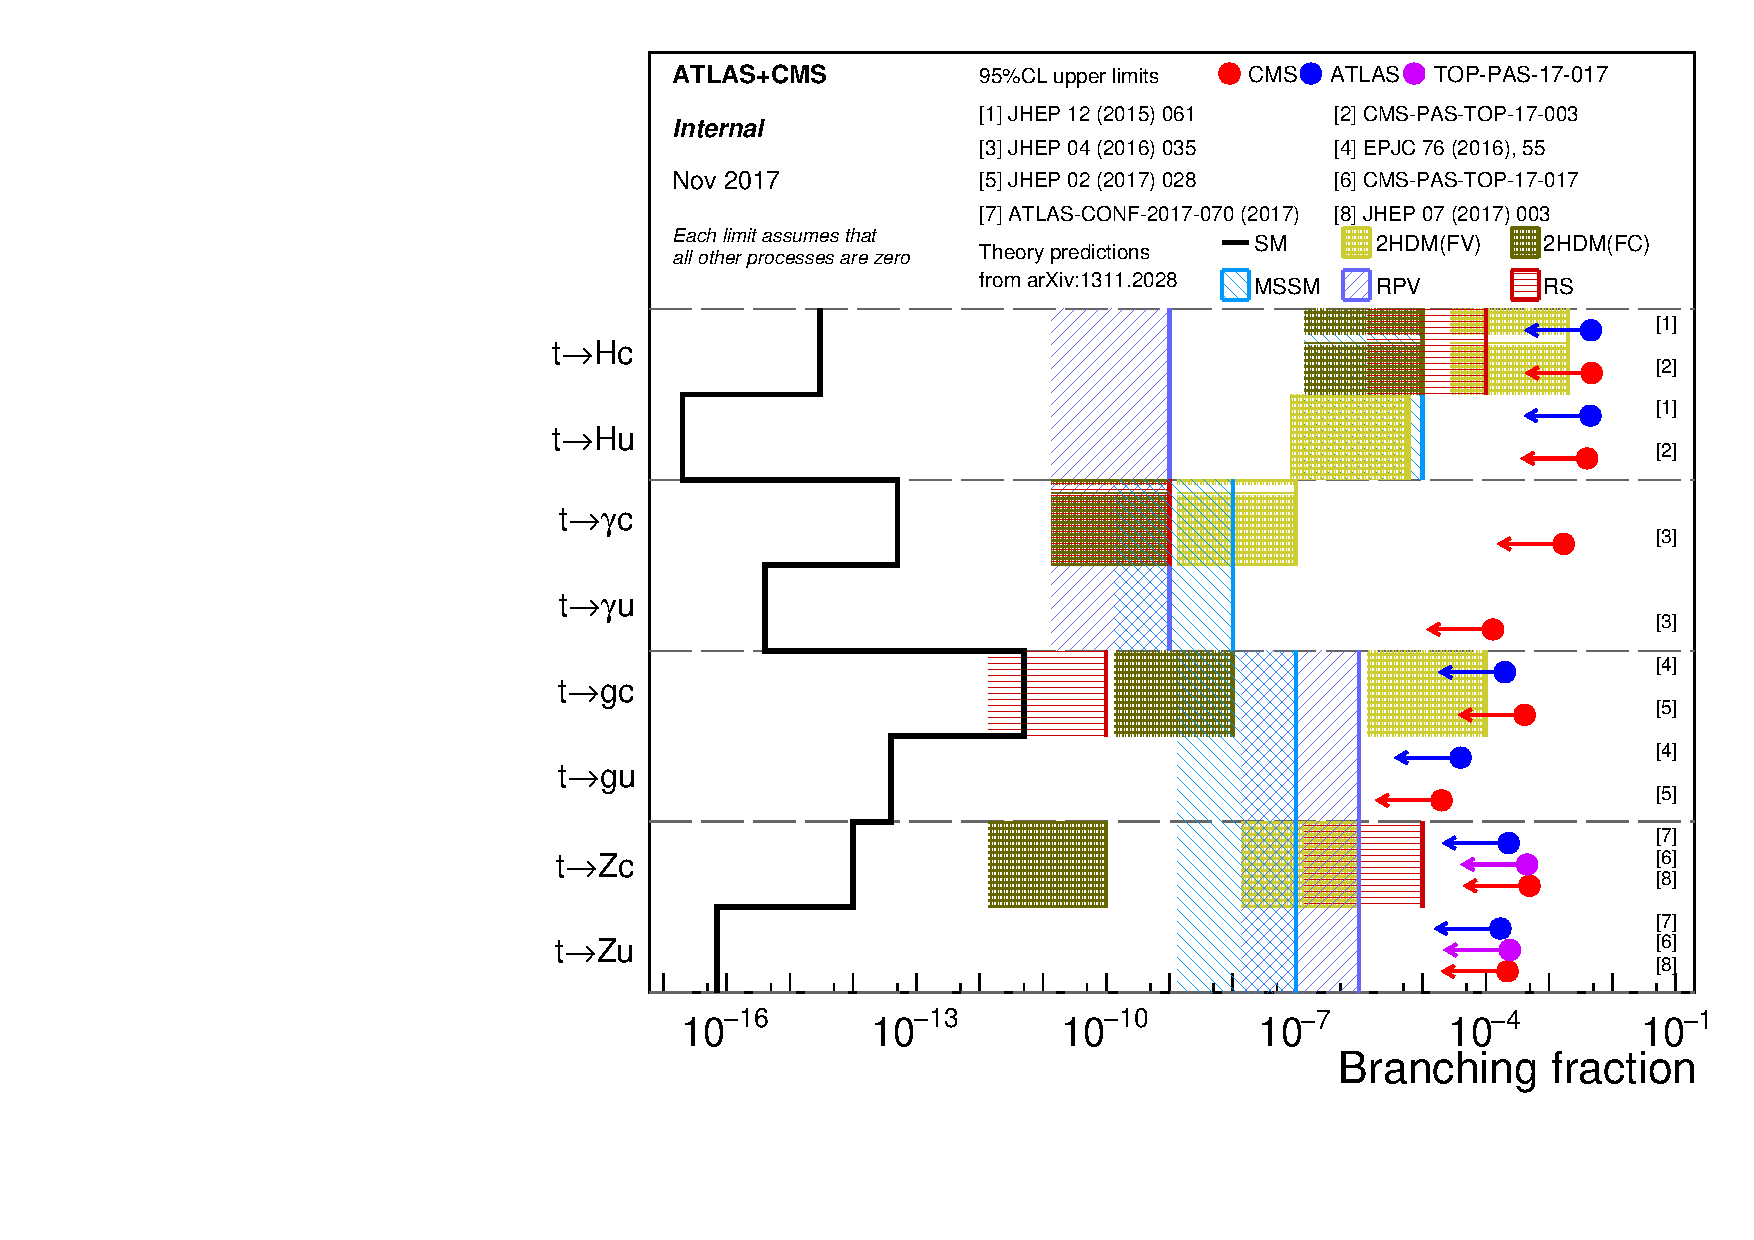
\includegraphics[width=0.7\linewidth]{7_Conclusion/Figures/fcnc_upperlimits.pdf}
%	\caption{Summary of the most stringent upper limits on top-FCNC interactions at 95\% CL upper limits from CMS (red) and ATLAS (blue) at a centre-of-mass of 8 and 13 \TeV. The results from this thesis are shown in purple. A comparison between theory predictions and experimental limits is shown. Figure adapted from \cite{summarywiki}.}
%	\label{fig:fcncupperlimitss}
%\end{figure}



\section{Prospects}
This statistically limited search is expected to have an improvement when performed on a larger dataset. By extrapolating the current analysis to a dataset of 100 \fbinv\ (full Run 2 dataset), 300 \fbinv\ (Run 2 + Run 3), or 3000 \fbinv\ (HL-LHC), keeping the systematic uncertainties as is,  the expected upper limits at 95\% CL are  extracted %. $\BR(\Ptop \rightarrow \Pup\PZ) < 0.0051\%$ and $\BR(\Ptop \rightarrow \Pcharm\PZ) < 0.014\%$
, assuming one non-vanishing coupling at a time. These limits, with respect to the result obtained in the presented search, are shown in \fig{fig:proj}.  An improvement with a factor 0.3 for the \Zut, and 0.4 for the \Zct\ vertex is expected for 100 \fbinv. For 300 \fbinv\ and 3000 \fbinv, this improves even more and certain beyond the Standard model theories could be confirmed or excluded. Setting statistical limitations aside, the largest systematic uncertainty is coming from the jet energy scale uncertainty. This uncertainty can be decreased by more precise measurements of the jet energy respond with more data as well as better methodologies. %A  calorimeter could help reducing the uncertainty.  % ook better handle op pu sinds hiervoor gecorrigeerd wordt
\begin{figure}
	\centering
	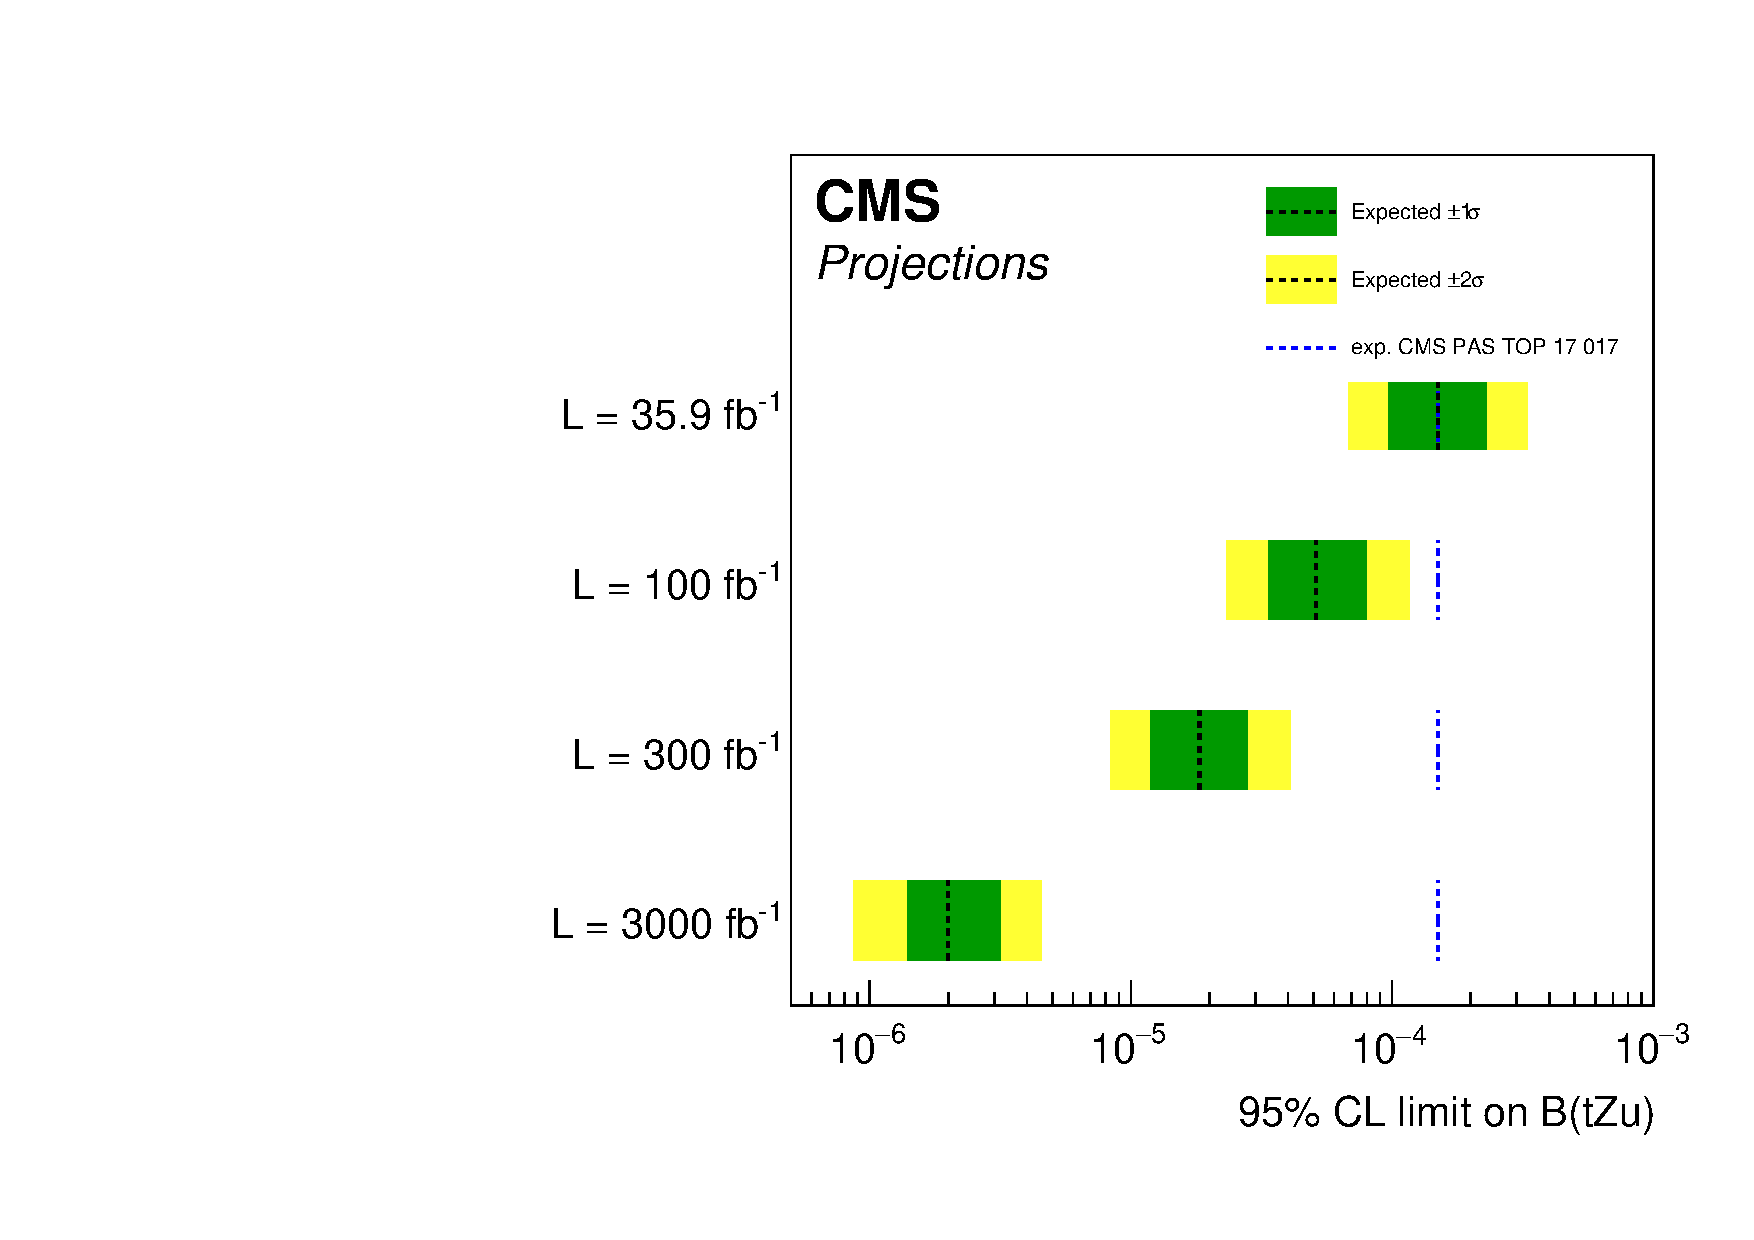
\includegraphics[width=0.49\linewidth]{7_Conclusion/Figures/TOP-17-017_limitsZutProj.pdf}
	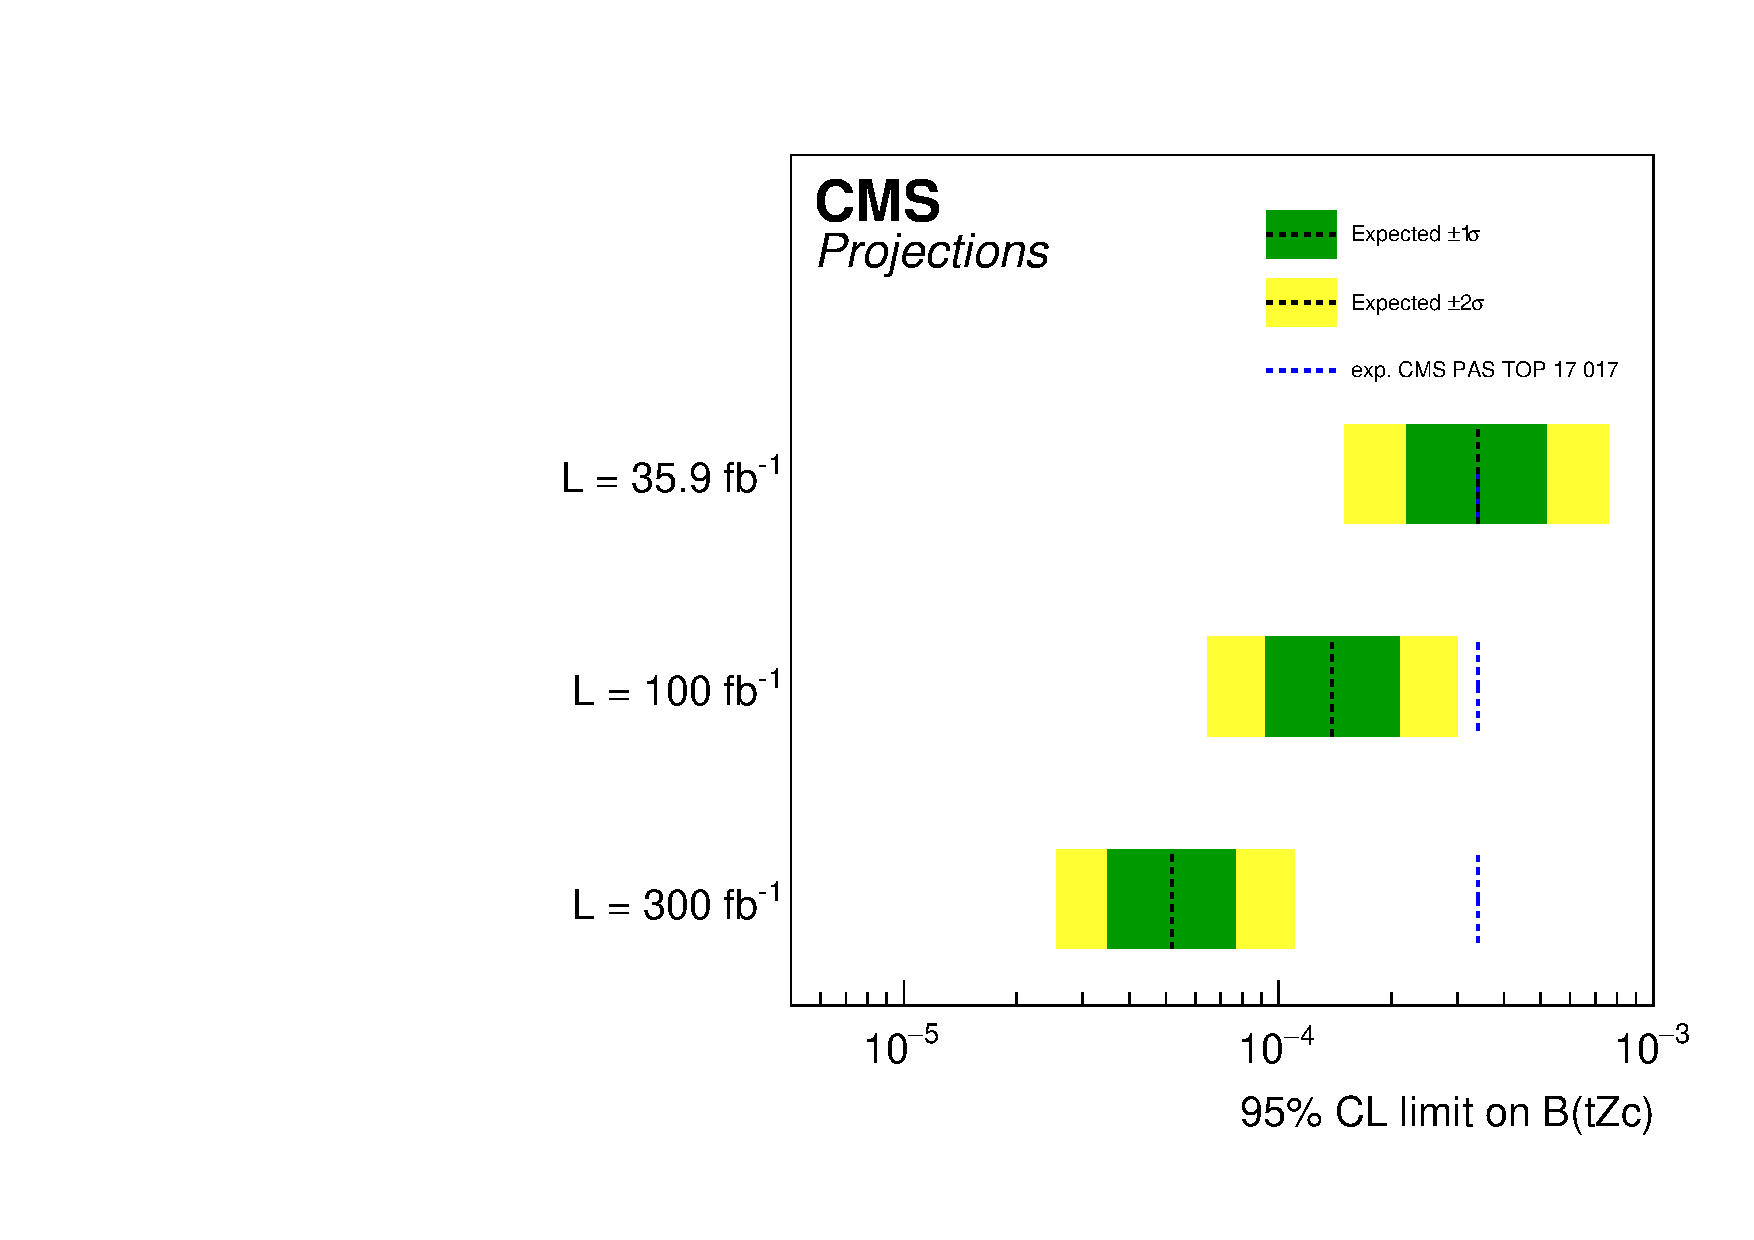
\includegraphics[width=0.49\linewidth]{7_Conclusion/Figures/TOP-17-017_limitsZctproj.pdf}
	\caption{The expected limit at 95\% CL for the \Zut\ (left) and \Zct\ interaction for an integrated luminosity of 100; 300, and 3000 \fbinv, extrapolated from the result obtained in this thesis, indicated with the blue (dashed) lines. }
	\label{fig:proj} % /user/ivanpari/CMSSW_8_0_26_patch1/src/TopBrussels/FCNCAnalysis > python limitsprj.py 
\end{figure}


The recently developed charm tagging algorithm could help the lesser sensitive FCNC signal with a \Zct\ vertex from its backgrounds. Additionally, a new pixel detector is installed in March 2017 and this is expected to enhance the performance of heavy-flavour tagging which should help improve the analysis. 

\newpage
Future colliders should be able to reach meaningful sensitivity for top-FCNC couplings. In \fig{fig:fcncupperlimitproj}, the sensitivity of the LHC at a centre-of-mass energy of 14 \TeV\ and 3000 \fbinv\ integrated luminosity (HL-LHC)~\cite{Agashe:2013hma}, as well as ILC/CLIC at a centre-of-mass energy of 500~\GeV\ and 500~\fbinv\ of integrated luminosity~\cite{Mangano:2016jyj}, the  future circular hadron colliders at a centre-of-mass of 100 \TeV\ with an integrated luminosity of 10 ab$^{-1}$ (FCC-hh)~\cite{Agashe:2013hma}, the future circular electron positron colliders at a centre-of-mass of 500~\GeV\ with an integrated luminosity of 10~ab$^{-1}$ (FCC-ee)~\cite{Khanpour:2014xla}, and the future Large hadron electron collider (LHeC) with a centre-of-mass of 14 \TeV\ and an integrated luminosity of 200 \fbinv~\cite{Liu:2015kkp} are shown. The sensitivities are originating from projections as well as sensitivity studies based on the changes in luminosity, energy, and trigger thresholds. 
\begin{comment}
The future large scale circular electron-positron collider (FCC-ee) would be one of the high- precision and high-luminosity machines which will be able to perform precise measurements on the Higgs boson, top-quark, Z and W bosons [43, 55]. Due to the expected large amount of data and large production rates, FCC-ee can provide an excellent opportunity for precise studies, in particular in the top quark sector. FCC-ee is designed to be working at the center-of-mass energy up to the tt ̄ threshold mass, i.e. √s = 350 GeV which is upgradeable to 500 GeV. The goal is to reach to a luminosity of L = 1.3 × 1034 cm−2s−1 [43, 55].
https://arxiv.org/pdf/1408.2090.pdf met feynman diagram

LHeC met feynman diagram https://arxiv.org/pdf/1507.03264.pdf

CLIC arXiv:1604.08122 en https://arxiv.org/pdf/1611.04492.pdf https://arxiv.org/pdf/1604.08122.pdf

HL LHC http://iopscience.iop.org/article/10.1088/1742-6596/706/2/022002/pdf

uitleg BSM model https://arxiv.org/pdf/1311.2028.pdf  (snowmass)

Kirill https://indico.cern.ch/event/659310/contributions/2690162/attachments/1527542/2389404/kskovpenTOP2017.pdf

atlas thesis https://cds.cern.ch/record/2272850/files/CERN-THESIS-2016-313.pdf
\end{comment}
\begin{figure}[htbp]
	\centering
	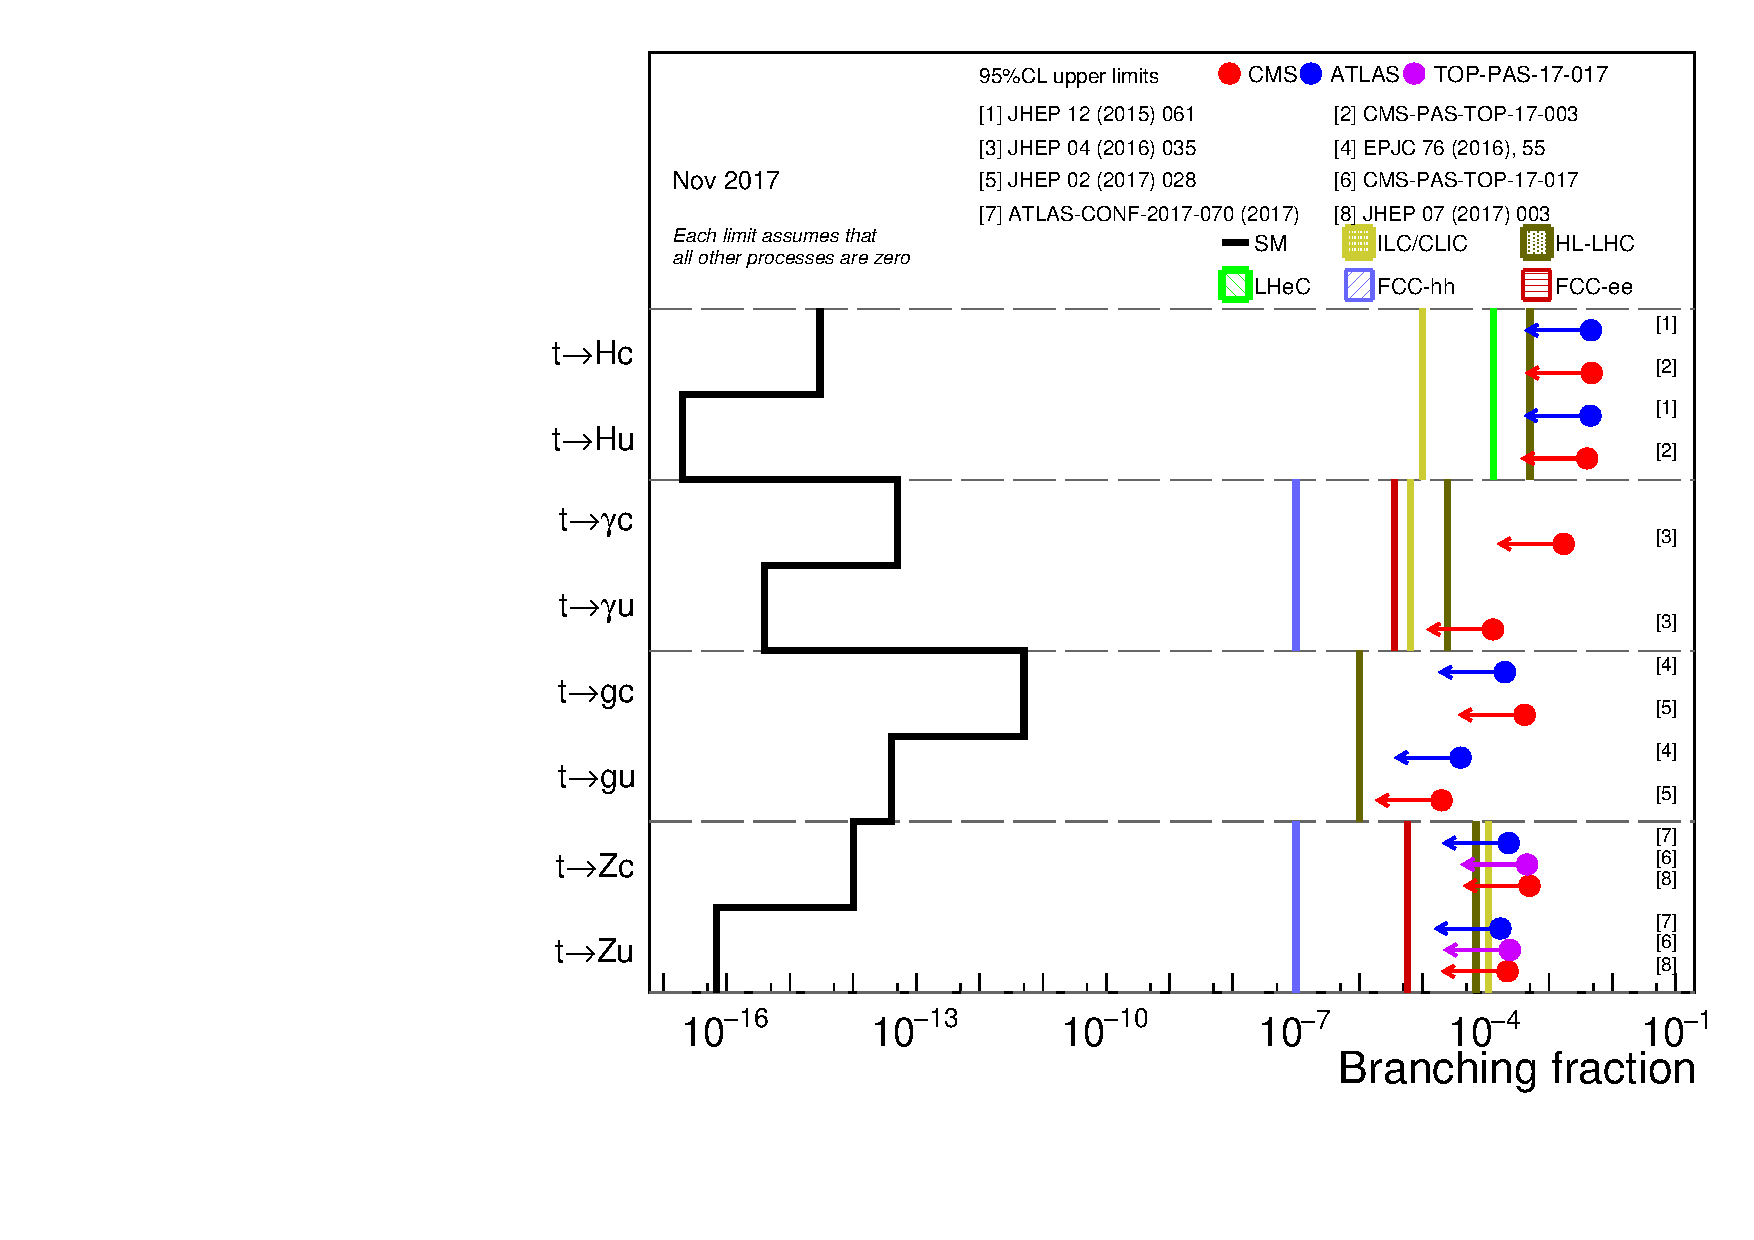
\includegraphics[width=1. \linewidth]{7_Conclusion/Figures/fcnc_upperlimits_proj.pdf}
	\caption{Summary of the most stringent upper limits on top-FCNC interactions at 95\% CL upper limits from CMS (red) and ATLAS (blue) at a centre-of-mass of 8 and 13 \TeV. The results from this thesis are shown in purple. A comparison between the projections for future colliders and the current experimental limits is shown. Figure adapted from \cite{summarywiki}. The projections are taken from \cite{Liu:2015kkp,Agashe:2013hma,Khanpour:2014xla,Mangano:2016jyj}.}
	\label{fig:fcncupperlimitproj}
\end{figure}


The HL-LHC is not expected to have significant improvements for the limits of the top-Z FCNC interactions. Instead of hadron colliders, one could also look at future lepton colliders such as the FCC-ee, where the signal $\Pep\Pem \rightarrow \PZ/\Pgamma \rightarrow \Ptop \APquark \: (\APtop\Pquark)$ can occur.  The FCC-ee would be one of the high luminosity and high precision machines and would be able to perform precise measurements of the top quark, Higgs, \PZ\, and \PW\  bosons. Its large production rates create an excellent environment for precise studies in the top quark section  of the Standard Model. In Ref. \cite{Khanpour:2014xla} a study of the FCNC \tZq\ single top quark production is done at different centre-of-mass energies and for different integrated luminosities. In \fig{fig:fcncupperlimitproj}, their most stringent results are shown. 

%\begin{figure}
%	\centering
%	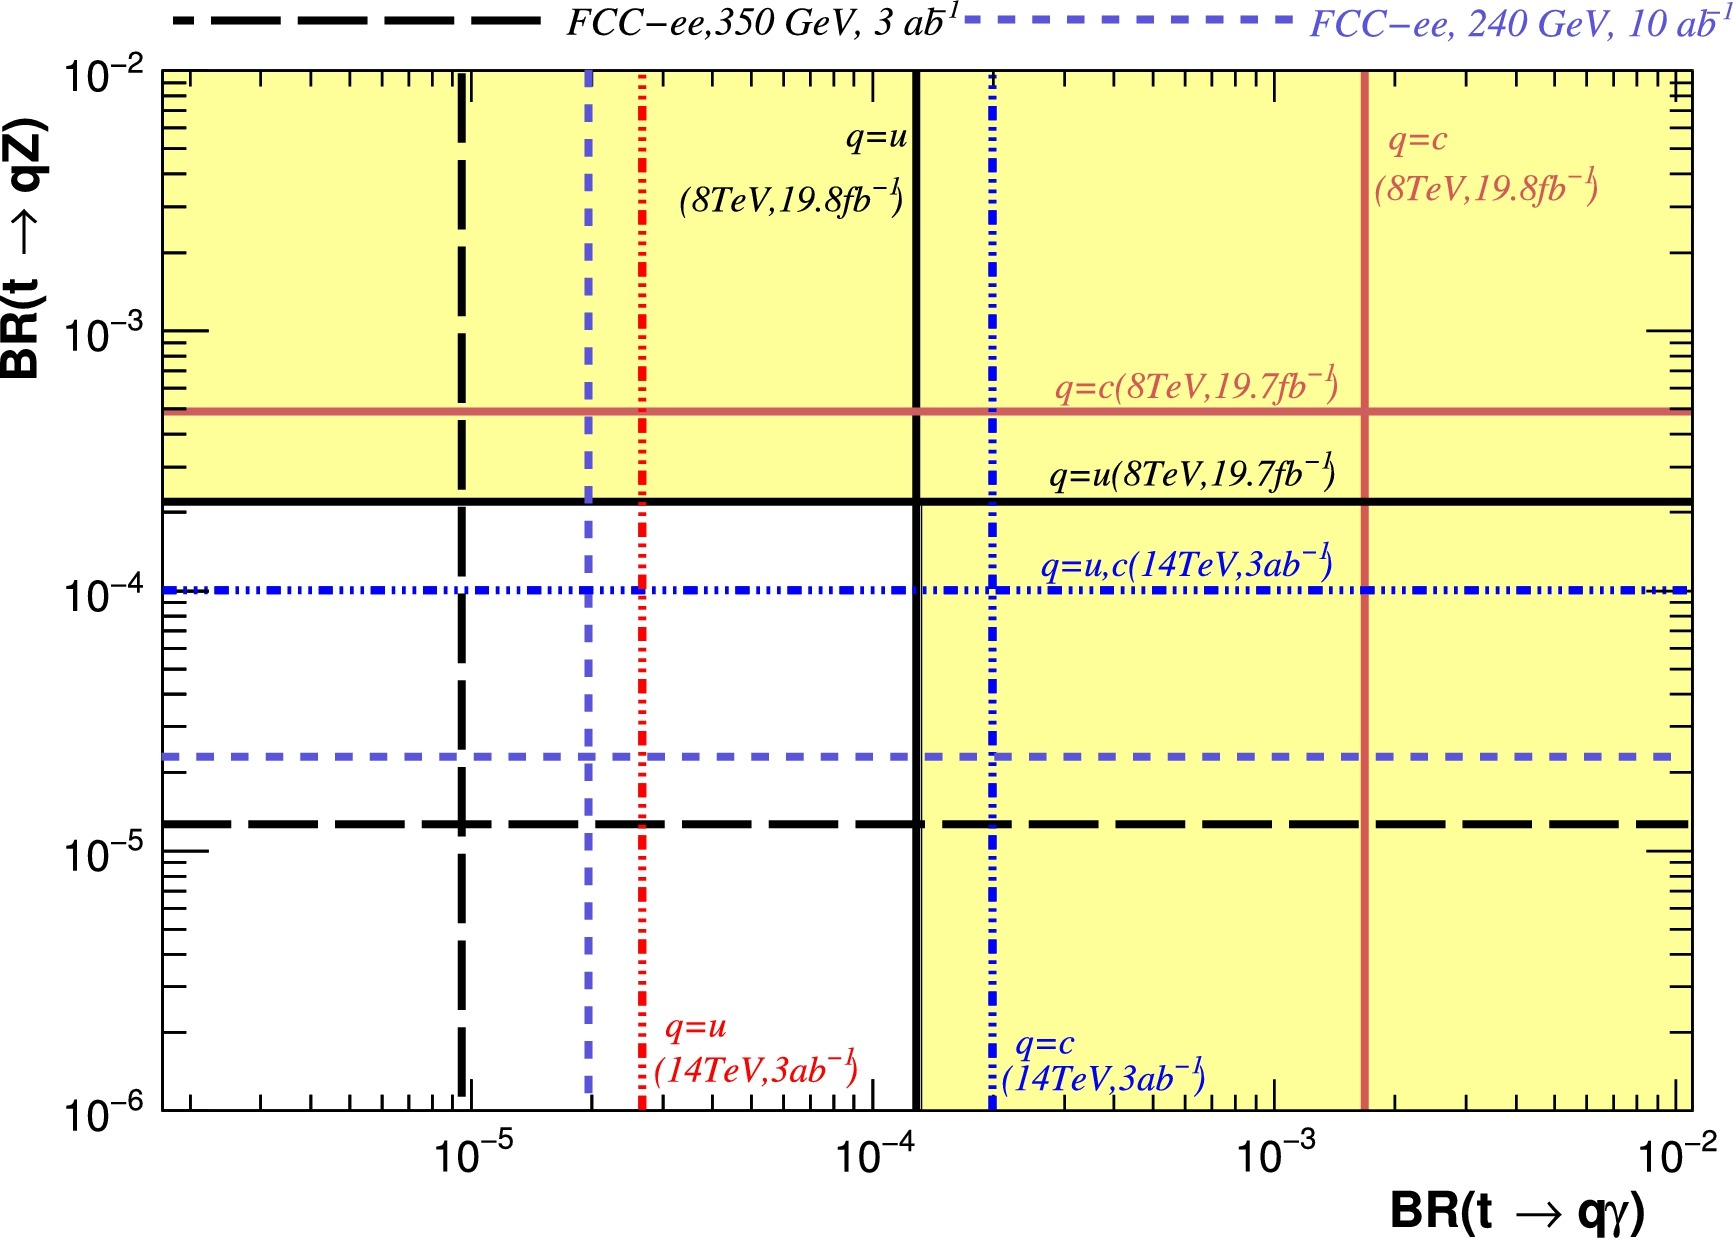
\includegraphics[width=0.49\linewidth]{7_Conclusion/Figures/FCCee}
%	\caption{The observed upper limits on the Br(t → qZ) versus Br(t → qγ) at 95% C.L from the recent analyses of the CMS experiment [13,27]. The expected sensitivity from the CMS experiment with 3000 fb−1 is also shown [30]. The sensitivity of the FCC-ee with 3 ab−1 at the center-of-mass energy of 350 GeV, and with 10 ab−1 at the center-of-mass energy of 240 GeV are presented as well. For the FCC-ee case, at a time one coupling is considered.}
%	\label{fig:fccee}
%\end{figure}
